\documentclass[amsmath,amssymb,notitlepage,11pt]{revtex4}
%\documentclass[12pt]{article}
\usepackage[toc,page]{appendix}
\usepackage{graphicx}
\usepackage{bm}% bold math
\usepackage{multirow}
\usepackage{booktabs}
\usepackage{verbatim}
\usepackage{hyperref}
\usepackage{enumitem}
\hypersetup{pdftex,colorlinks=true,allcolors=blue}
\usepackage{hypcap}
\usepackage[small,compact]{titlesec}
\setlist[enumerate]{itemsep=0mm}

\begin{document}
\title{CLAS12 M{\o}ller Operations Manual - v0.0}
\date{\today}
\author{N. Baltzell}
\begin{abstract}
\end{abstract}

\maketitle
%\tableofcontents
%\newpage

\section{Introduction}
The CLAS12 M{\o}ller system measures the longitudinal polarization of the electron beam delivered to Hall B, and this document details its operating procedures.  The user interface for shift workers is shown in Fig.~\ref{fig:run} and provides direct access to all controls and feedback that the normal operator should need, described in Section~\ref{sec:user}.  Expert operations are described in Section~\ref{sec:expert}.


\begin{figure}[htbp]\centering
    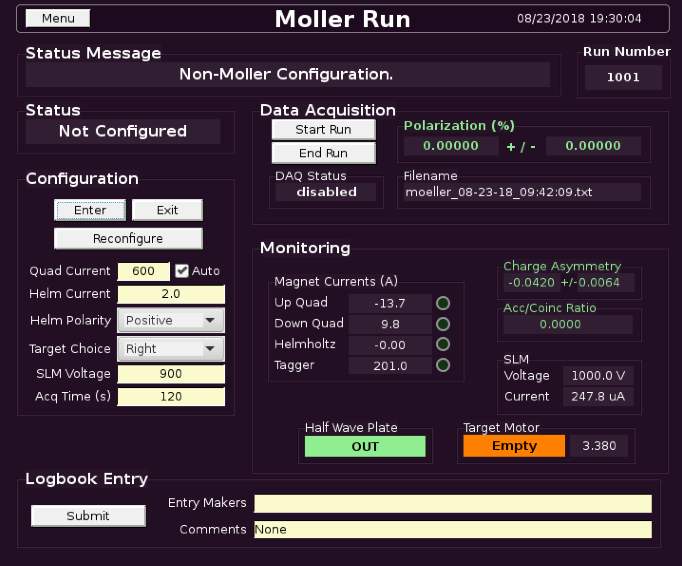
\includegraphics[width=11cm]{pics/run}
    \caption{The user interface for shift workers for operating a M{\o}ller run.\label{fig:run}}
\end{figure}


\section{Standard Procedures}\label{sec:user}
The instructions for the automated procedure.

\section{Expert Procedures}\label{sec:expert}
The instructions for the old, manual procedure.

\newpage
\begin{appendices}
Description of the hardware and software involved in the CLAS12 M{\o}ller system.
\subsection{Quadrupoles}
\subsection{Helmholtz}
\subsection{Synchrotron Light Monitor}
\subsection{Target}
\subsection{Helicity Signal}
\subsection{Multi-Channel Scaler}
\subsection{EPICS IOCs}
\end{appendices}

\end{document}

